\section{Provisioning}
\label{fundamentals:provisioning}

This section provides an overview of provisioning in the context of computing.
First, we present a general introduction and describe some of the provisioning solutions available today.
Then, we focus in particular on TOSCA and OpenTOSCA because those are used in the prototypical implementation later on.

\subsection{Overview}

Setting up a complex distributed system with many different components scattered across multiple environments is a time-consuming task if done by hand.
For this reason, many provisioning solutions have been created over the years to automate this process.
They differ in some areas, but their core functionality is basically identical: They prepare all necessary resources for a certain task.
This core functionality can be stated more precisely with the following definition: Provisioning is, "in telecommunications, the setting in place and configuring of the hardware and software required to activate a telecommunications service for a customer; in many cases the hardware and software may already be in place and provisioning entails only configuration tasks"~\autocite{def:provisioning}.
Because we are working in a cloud environment, we will not have to deal with hardware directly, but rather with \nom{virtual machines}{VMs}.
So for us, provisioning means the creation and deletion of VMs in a cloud environment, as well as the installation, configuration, monitoring, running and stopping of software on these VMs~\autocite{provisioning:architecture}.

There are many benefits to using an automated provisioning solution instead of doing the provisioning by hand.
The manual approach is limited by how much work a single person can do at any time, whereas an automatic approach is able to do much more work, in less time, and potentially in parallel.
This makes it possible to manage huge infrastructures with very little resources, which can save time and money compared to a manual approach.
As every step that needs to be done to provision a system has to be written down, a detailed description of the whole provisioning process is created.
This makes the whole process reproducible and less error-prone, because the human factor is largely replaced by automation.
Parts of such a description can also be shared in a business or even between businesses, which makes the process of creating such a description potentially much more efficient.

The general process of working with provisioning software is very similar with all the different solutions.
It can be described as a two step process.
In step one, a description of the whole provisioning process has to be created using the tools provided by the particular solution.
In general, this involves creating a textual description in a certain format that is understood by the provisioning software that is to be used.
In this description, we tell the software what virtual resources we need, what software should be installed on them and how everything should be configured.
In step two, we pass this description to the provisioning software which interprets and executes it.

Many different provisioning solutions exist today.
Some cloud providers offer provisioning solutions that are particularly tailored to their cloud offerings, for example AWS CloudFormation\footnote{\url{http://aws.amazon.com/cloudformation}}, which can only be used to provision resources in the Amazon cloud.
Then, there are more generally usable provisioning solutions that are not bound to any particular cloud provider.
A few popular examples include Ansible\footnote{\url{http://www.ansible.com}}, Chef\footnote{\url{http://www.getchef.com/chef}}, Puppet\footnote{\url{http://puppetlabs.com/}}, and TOSCA\footnote{\url{https://www.oasis-open.org/committees/tc_home.php?wg_abbrev=tosca}}, which we will discuss in detail later.

All these solutions differ in some form or another.
A full feature comparison of different solutions is out of scope for this diploma thesis, but what follows is a short overview of some of the differences.
As already mentioned, AWS CloudFormation is bound to Amazon's cloud platform, while the other solutions are not.
Chef and Puppet both use a client server architecture, where each node that should be configured by them has to run a client program to communicate with a server node, whereas Ansible executes its command over \nom{Secure Shell}{SSH} and therefore does not require additional software on the nodes that are configured.
The solutions also differ in modularity and flexibility. While Ansible, Chef, Puppet, and TOSCA are highly flexible and can be used in a fine grained modular fashion, this also makes them more complex to use, for example compared to AWS CloudFormation.

\subsection{TOSCA}

\nom{Topology and Orchestration Specification for Cloud Applications}{TOSCA} is a standard created by the \nom{Organization for the Advancement of Structured Information Standards}{OASIS}\footnote{\url{https://www.oasis-open.org/}}~\autocite{tosca:spec}.
Its development is also supported by various industry partners, which include IBM, Cisco, SAP, HP and others.
Its aim is to provide a language that can describe service components and their relations in a cloud environment independent fashion.
The following description is based on version 1.0 of the specification~\autocite{tosca:spec}.

TOSCA defines an XML syntax, which describes services and their relations in a so called service template.
All elements needed to define such a service template are provided in the TOSCA definitions document.
\autoref{image:tosca:definitions} shows such a definitions document.
Aside from the actual service template, shown on the left, it also contains a number of type definitions and some templates based on those definitions.
These definitions and templates can also be imported from a separate definitions document.

\begin{figure}[!htbp]
	\centering
	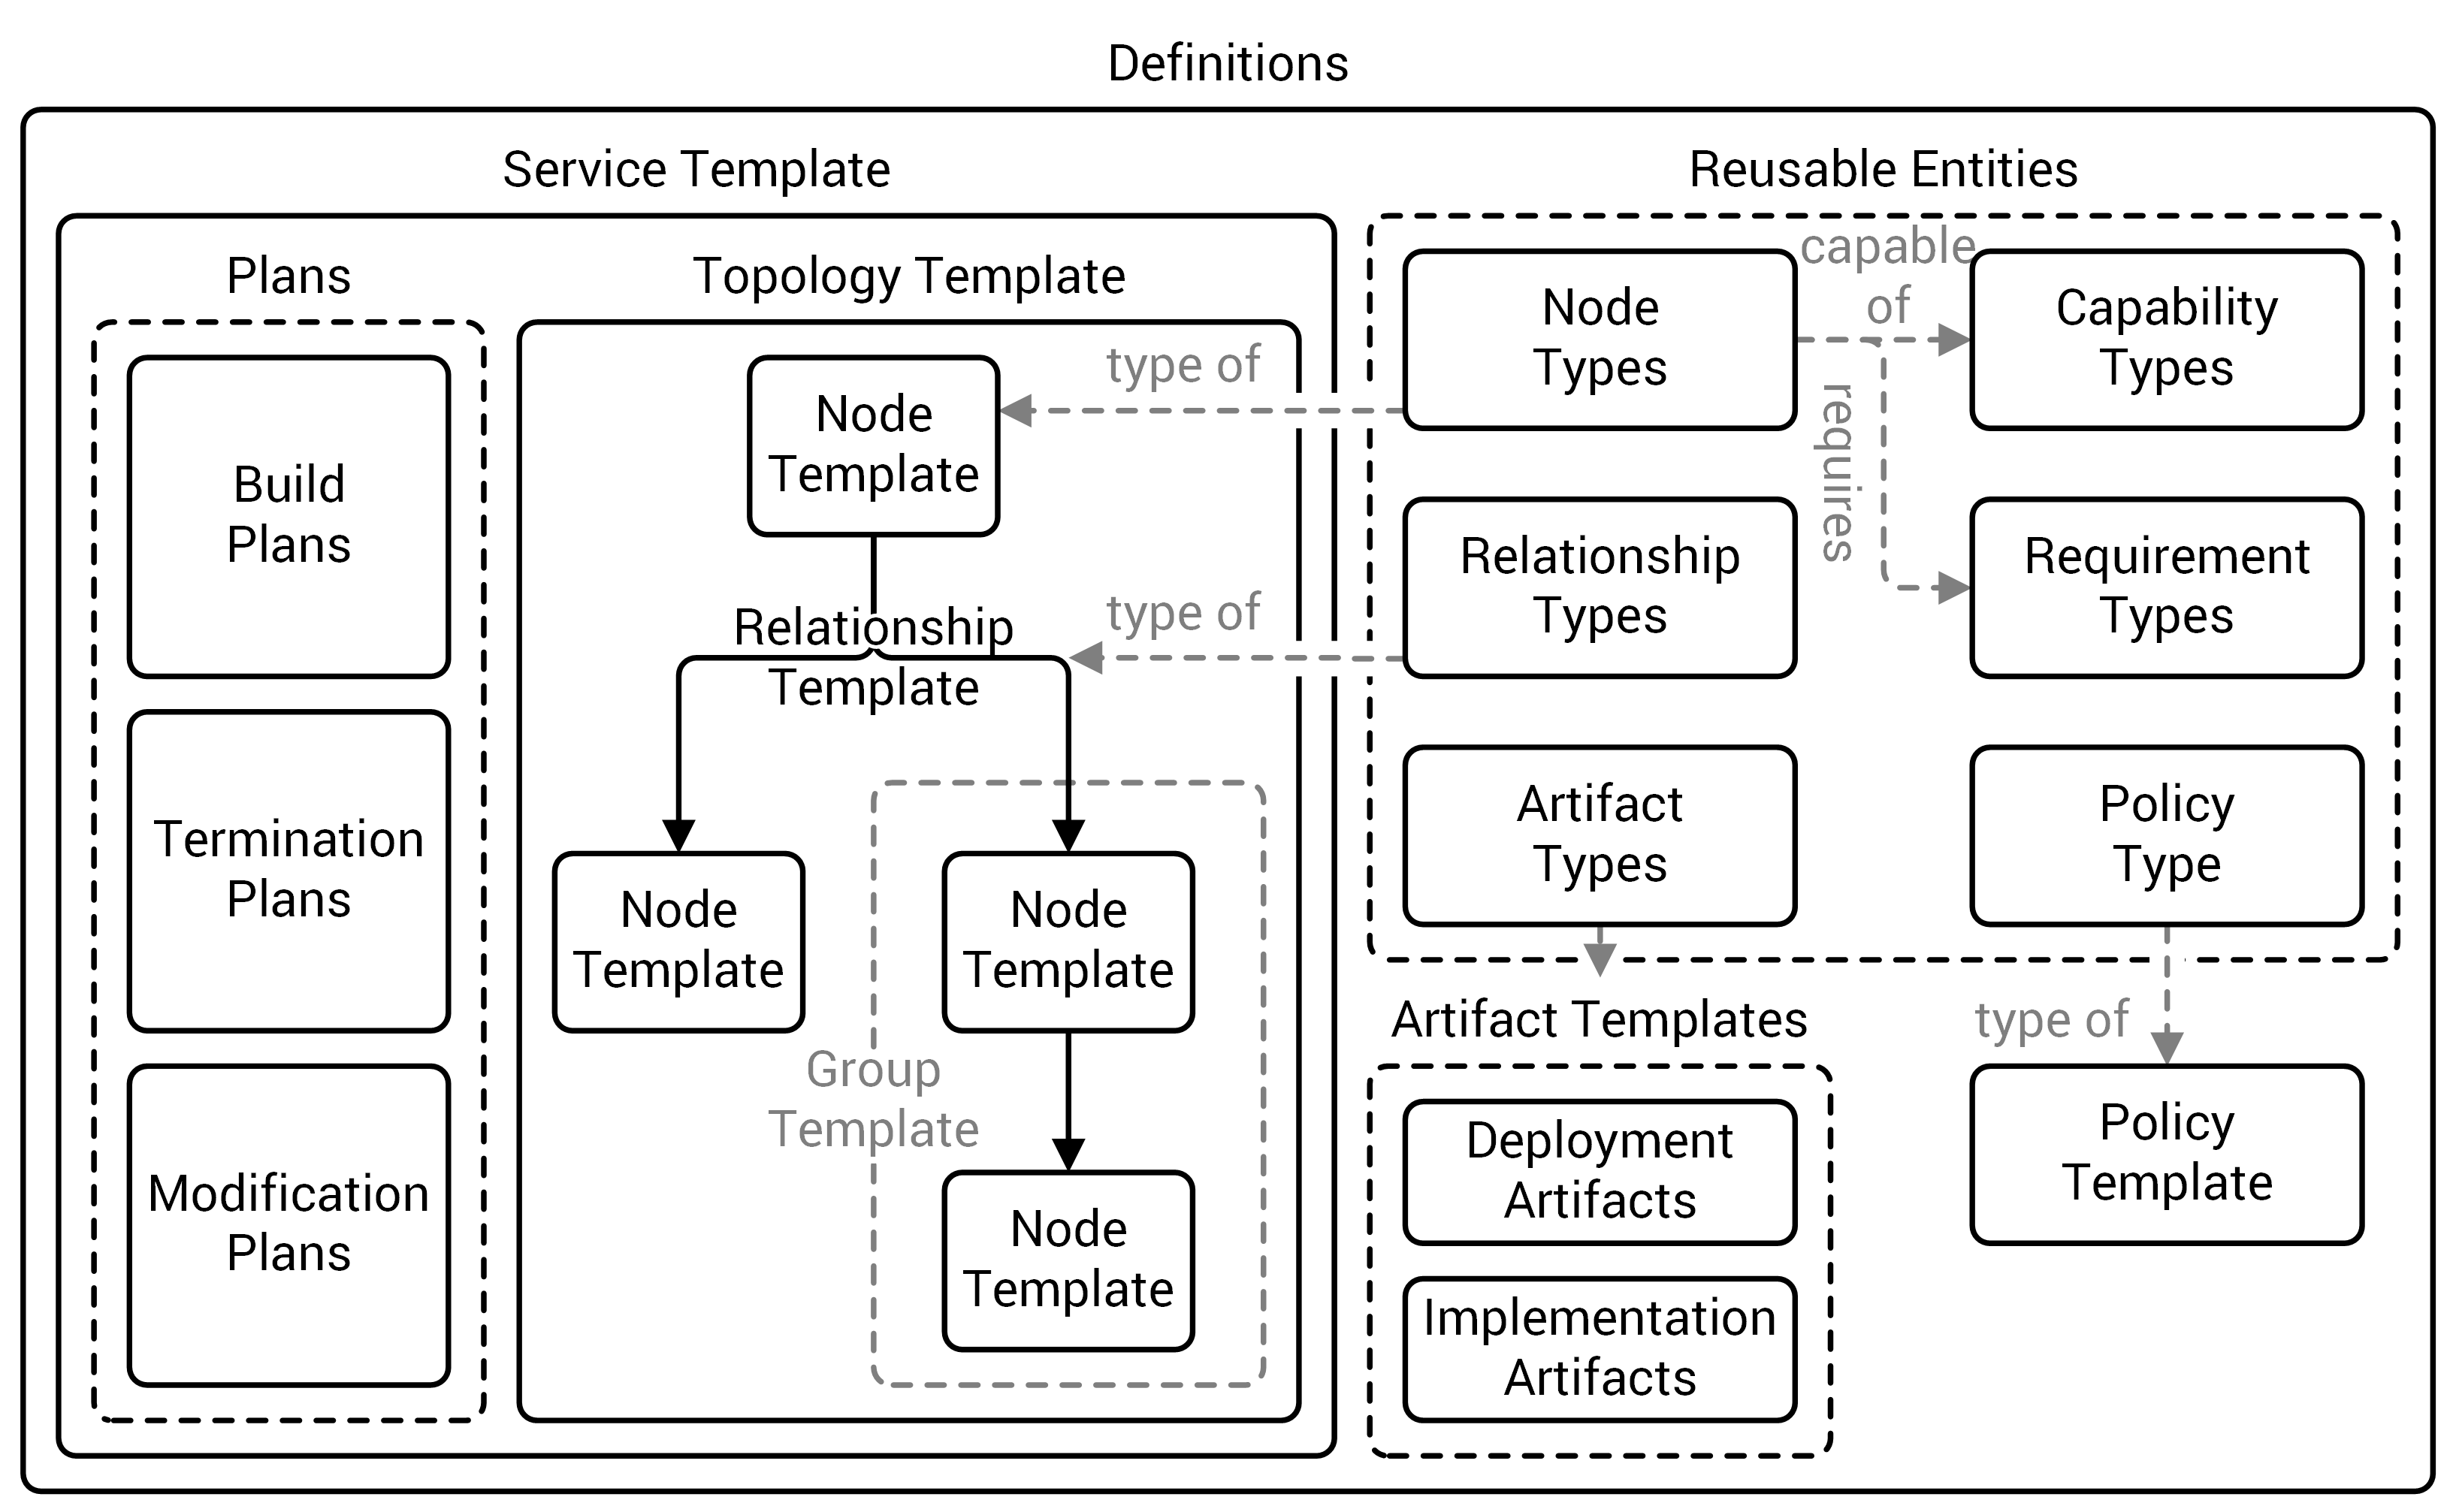
\includegraphics[resolution=600]{fundamentals/assets/definitions}
	\caption{TOSCA definitions structure~\autocite[based on][]{tosca:spec}.}
	\label{image:tosca:definitions}
\end{figure}

The service template consists of two parts: A topology template and plans.
Topology templates, as seen in the center of \autoref{image:tosca:definitions}, model the structure of a service and the middleware and infrastructure supporting it as a directed graph.
The vertices of the graph represent nodes which are occurrences of a specific component, for example, an application server or a database.
These nodes are defined by node types or by other service templates.
Node types are reusable entities, as shown in the top right of \autoref{image:tosca:definitions}.
They define the properties of a component, as well as operations to manipulate a component, so called interfaces.
Additionally, node types can be annotated with requirements and capabilities.
These, in turn, are defined by requirement and capability types, which also belong to the group of reusable entities.
This allows for requirement and capability matching between different components.
The edges of the graph represent connections between nodes, which are defined by relationship templates that specify the properties of the relation.
An example for such a connection would be a node A, representing a web service that is deployed on node B, an application server.
Relationship types are also used to connect requirements and capabilities.

Plans, shown on the left of \autoref{image:tosca:definitions}, are used to manage the service that is defined by the service template. TOSCA distinguishes between three types of plans: Build plans, termination plans, and modification plans.
Build plans describe how instances of a service are created.
Termination plans describe how such a service is removed.
Modification plans manage a service during its runtime.
These plans consist of one or more tasks, i.e. an operation on a node (via an interface) or an external service call, and the order in which these tasks should be performed.
They can be written in a process description language like \nom{Business Process Execution Language}{BPEL}\footnote{\url{http://docs.oasis-open.org/wsbpel/2.0/OS/wsbpel-v2.0-OS.html}} or \nom{Business Process Modeling Notation}{BPMN}\footnote{\url{http://www.bpmn.org/}}.

The bottom right of \autoref{image:tosca:definitions} shows artifact templates which represent artifacts.
Artifacts are things that can be executed directly (e.g.: scripts, archives) or indirectly (e.g.: URL, ports).
TOSCA further distinguishes between two types of artifacts, namely deployment and implementation artifacts.
Deployment artifacts materialize instances of a node and are used by a build plan to create a service.
An example for this is an \nom{Amazon Machine Image}{AMI} which creates an Apache server once deployed in a VM.
Implementation artifacts implement the interfaces of components.
Here, an example would be a node that has an interface for starting the particular component described by the node.
This interfaces could be implemented by an implementation artifact like a \textit{.jar} file.

The bottom right of \autoref{image:tosca:definitions} also shows policy templates that refer to specific policy types.
A policy template can define concrete values for a policy specified in a policy type.
A node template can then reference a policy template to declare that it supports some non-functional properties or a certain kind of quality-of-service.
An example would be a node type for an application server that expresses that it supports high availability by referencing a matching policy template.

One or more TOSCA definitions are packaged, together with some metadata and possibly other files, into a \nom{Cloud Service Archive}{CSAR}, which is essentially a \textit{zip} file that contains all files necessary to create and manage a service.
CSAR files can then be executed in a TOSCA runtime environment, also called TOSCA container, to create the service described within.

\subsection{OpenTOSCA}

OpenTOSCA is a browser based open-source implementation of a TOSCA container, created at the IAAS at the University of Stuttgart, which supports the execution of TOSCA CSAR archives~\autocite{opentosca}.
\autoref{image:tosca:opentosca} shows the architecture of OpenTOSCA.
Its functionality is realized in three main components, which are the Controller, the Implementation Artifact Engine, and the Plan Engine.
After a CSAR is uploaded to OpenTOSCA it can be deployed in three steps.
In the first step, the CSAR file is unpacked and its content is stored for further use.
The TOSCA XML files are then loaded and processed by the Controller.
The Controller in turn calls the Implementation Artifact Engine and the Plan Engine.
The Implementation Artifact Engine knows how to deploy and store the provided implementation artifacts via plugins.
Plans are then run by the Plan Engine, which also uses plugins to support different plan formats.
OpenTOSCA also offers two \nom{application programming interfaces}{APIs}, the Container API and the Plan Portability API.
The Container API can be used to access the functionality provided by the container from outside and to provide additional interfaces to the container, like the already existing admin UI, self-service portal, or modeling tool.
The Plan Portability API is used by plans to access topology and instance information~\autocite{opentosca}.

\begin{figure}[!htbp]
	\centering
	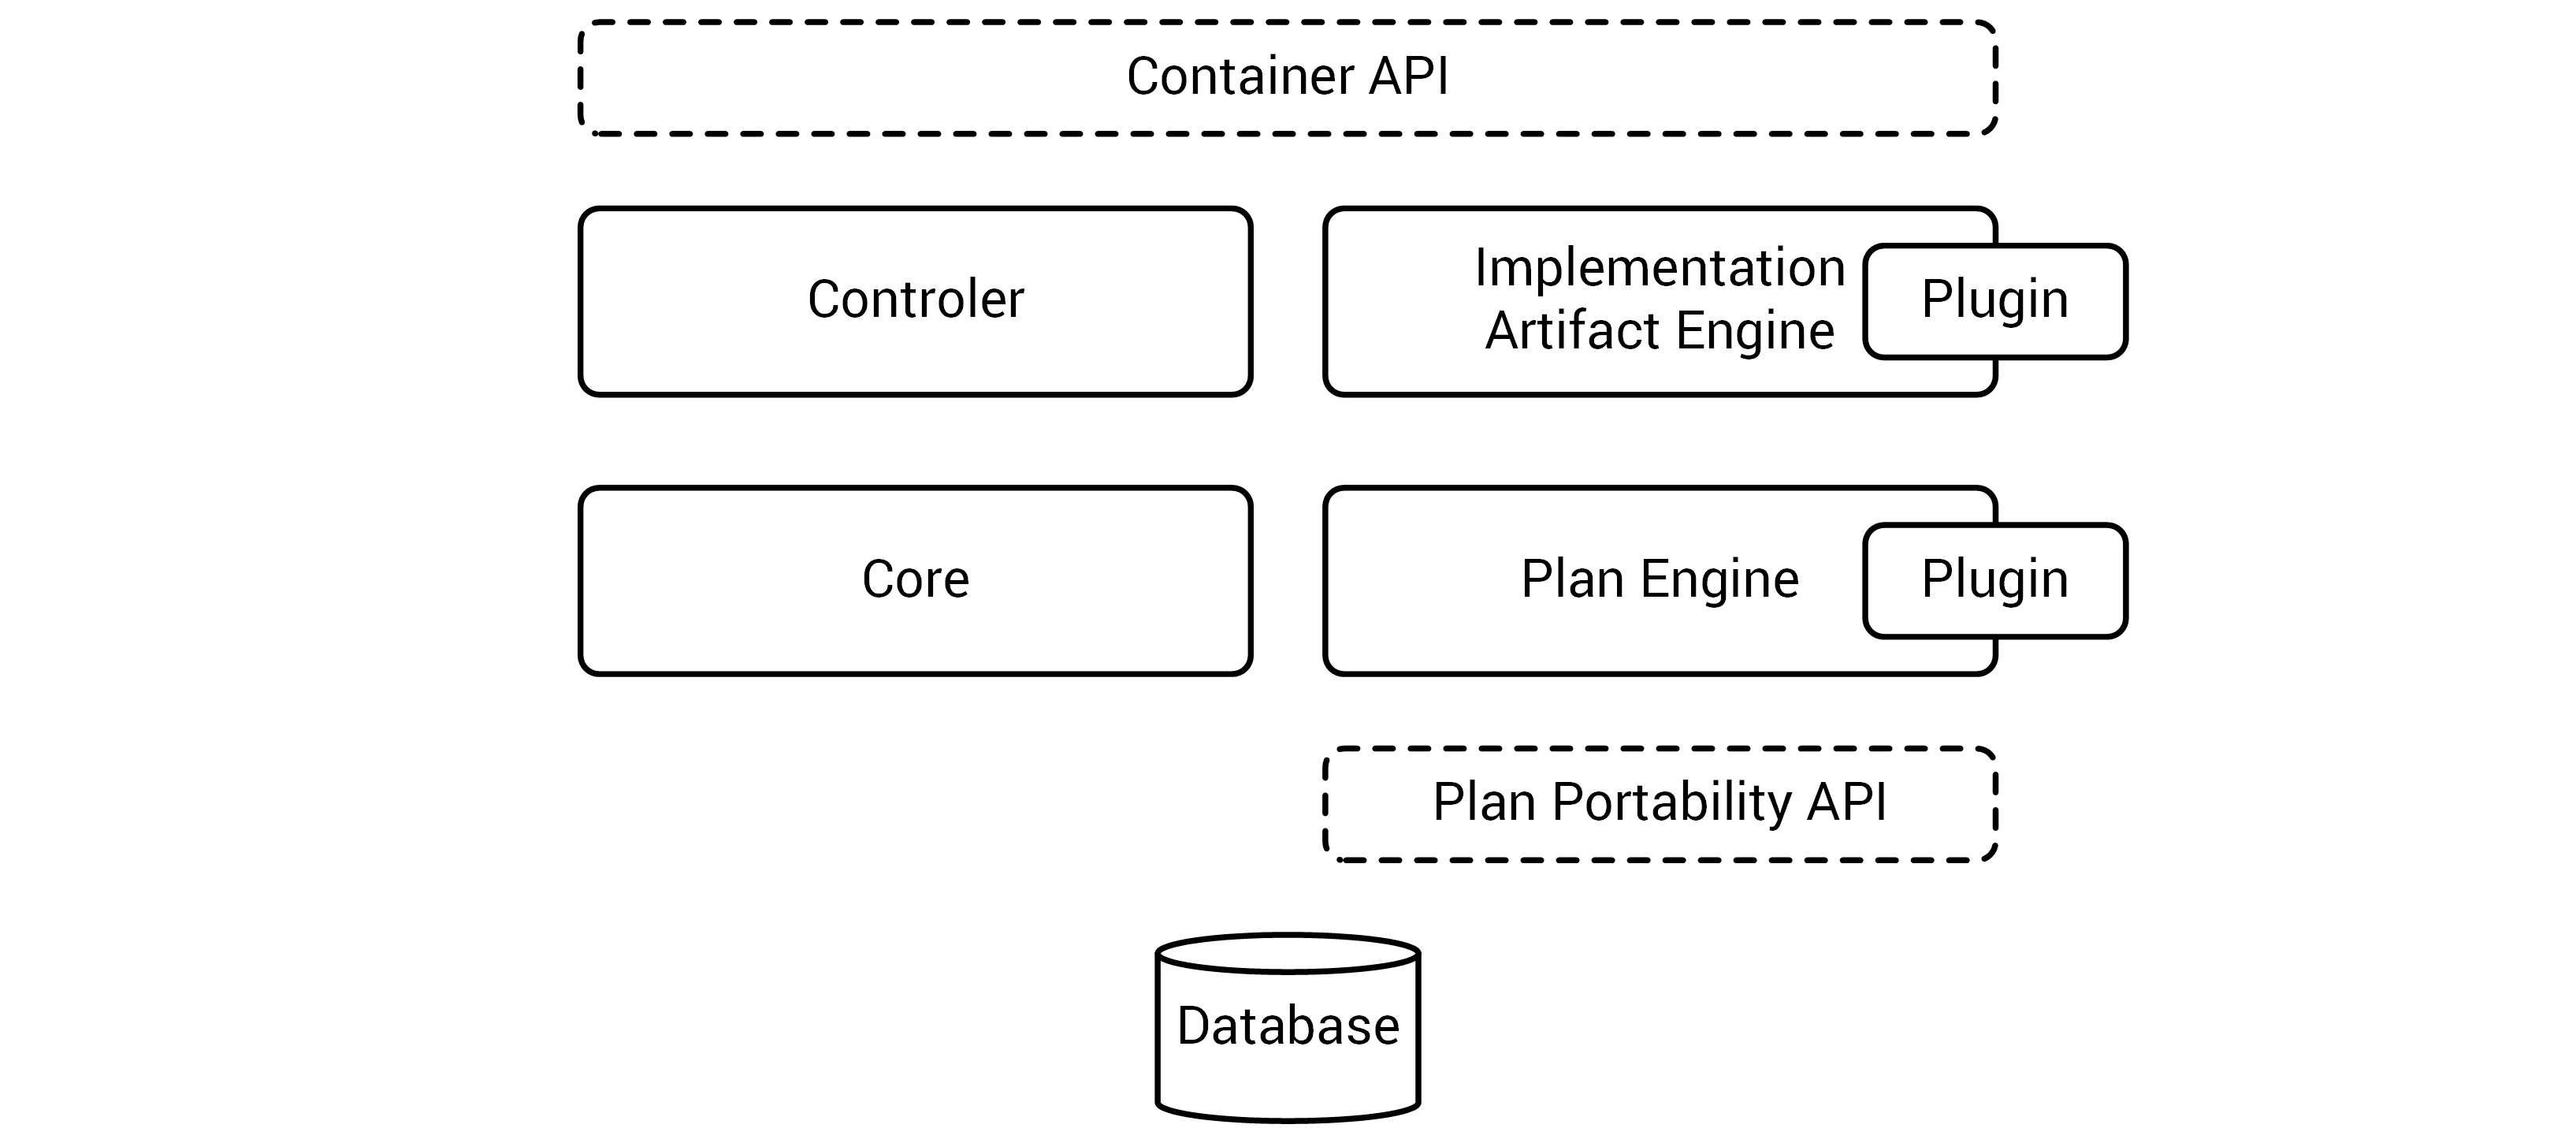
\includegraphics[resolution=600]{fundamentals/assets/opentosca}
	\caption{OpenTOSCA architecture~\autocite[based on][]{opentosca}.}
	\label{image:tosca:opentosca}
\end{figure}
